
\chapter{MajorMatch}

\section{The Interest Elicitation Problem}

% TODO: Add a sentence connecting this section to Chapter 3 -- the clustering work
% establishes that semantically coherent groupings exist; this section should explain
% why that structure is useful for interest elicitation specifically. Something like:
% the existence of meaningful clusters (Chapter 3) makes a cluster-first pipeline viable;
% without that, filtering by cluster would be arbitrary.

The fundamental goal of MajorMatch is to give students who do not know what they want to major in a starting place to explore. The challenge is not surfacing a ranked list: it is helping students articulate preferences they have not yet formed.

MajorMatch extends the TopProRec approach by replacing the open-ended topic browsing step with a more structured interest input. Rather than presenting students with a raw list of extracted keywords to sift through, MajorMatch guides them through a set of predefined dimensions that map to concrete aspects of academic programs. This reduces the cognitive burden of the interest elicitation step while preserving the core idea that a student's expressed preferences, not prior behavioral data, drive the recommendations.

\section{System Design}

% TODO: Add a figure here showing the two-stage pipeline (CLAUDE.md requires one).
% A simple flow diagram: student input -> Game 1 + 2 -> Stage 1 cluster selection ->
% Game 3 -> Stage 2 program selection -> ranked results with confidence scores.
% Reference it with \ref{fig:pipeline} or similar.

MajorMatch operates in two stages. Stage 1 uses responses to Games 1 and 2 to select the top 1--4 clusters that match the student's interests. Stage 2 uses Game 3 responses, combined with the Game 2 signal, to select up to 3 programs from each matched cluster, each with a confidence score.

\begin{figure}[h]
    \centering
    \missingfigure{Two-stage pipeline: student input $\to$ Games 1+2 $\to$ Stage 1 cluster selection $\to$ Game 3 $\to$ Stage 2 program selection $\to$ ranked results with confidence scores.}
    \caption{MajorMatch two-stage matching pipeline.}
    \label{fig:pipeline}
\end{figure}

% TODO: Add an interpretability paragraph here. The cluster-based design makes
% recommendations transparent in a way black-box collaborative filtering cannot:
% each output is traceable to a cluster match (Stage 1) and a keyword selection
% (Stage 2), so a student can see exactly why a program was surfaced. This is a
% meaningful design property worth stating explicitly -- it distinguishes MajorMatch
% from embedding-only nearest-neighbor approaches and connects to the broader thesis
% argument that explicit semantic structure (from clustering) adds value beyond
% raw embedding similarity.

The default dataset includes 106 popular majors across the United States, organized into 8 clusters: Law, Justice \& Public Policy; Creative Arts \& Media; Business \& Management; Engineering \& Technology; Health \& Behavioral Sciences; Sciences \& Mathematics; Education \& Teaching; and Humanities \& Cultural Studies. Full cluster descriptions appear in Appendix~\ref{app:clusters}.

% TODO: Explain how the 8 clusters were derived. Were they hand-authored, derived from
% the embedding clusters in Chapter 3, or a combination? This is a gap -- the reader
% will ask where these 8 groupings came from given that Chapter 3 used 23 CIP areas.

\section{Interest Elicitation via Structured Games}

MajorMatch collects student preferences through three games, each serving a distinct role in the matching pipeline.

\textbf{Game 1: Fact or Fiction} presents eight binary statements, one per cluster. Students mark each as true or false for themselves. Any cluster they reject is filtered out of the candidate set. The statements are designed to surface broad alignment with a field (see Appendix~\ref{app:games} for the full list).

\begin{figure}[h]
    \centering
    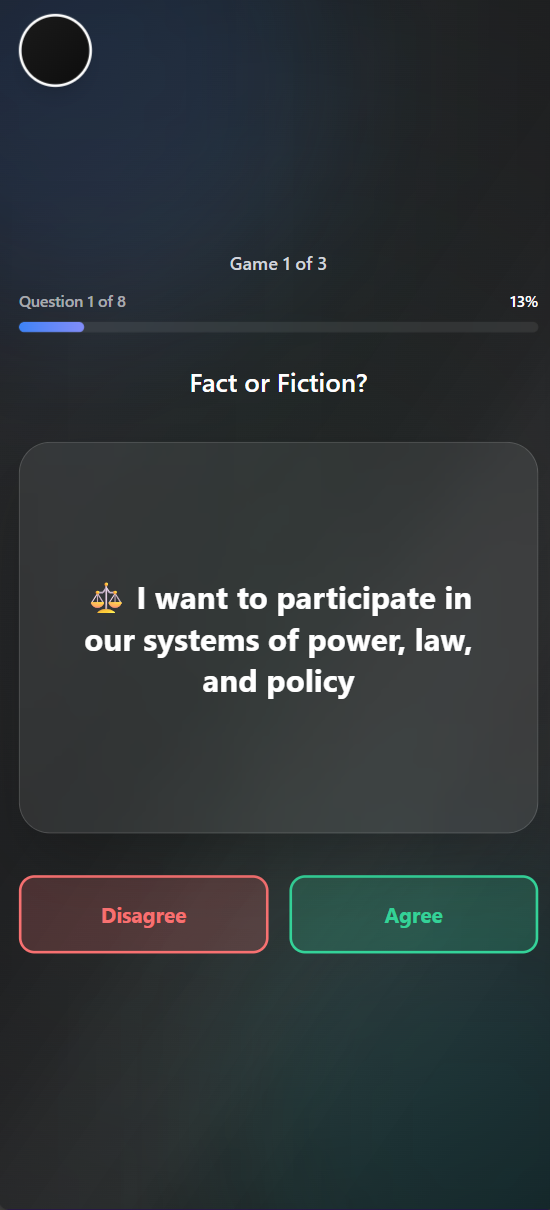
\includegraphics[width=0.75\textwidth,height=0.75\textheight,keepaspectratio]{Figures/game_1_fact_or_fic.png}
    \caption{Game 1: Fact or Fiction interface.}
    \label{fig:game1}
\end{figure}

\textbf{Game 2: This or That} presents nine forced-choice pairs that capture where a student falls on key academic dimensions. The student picks one option from each pair (see Appendix~\ref{app:games} for the full list).

\begin{figure}[h]
    \centering
    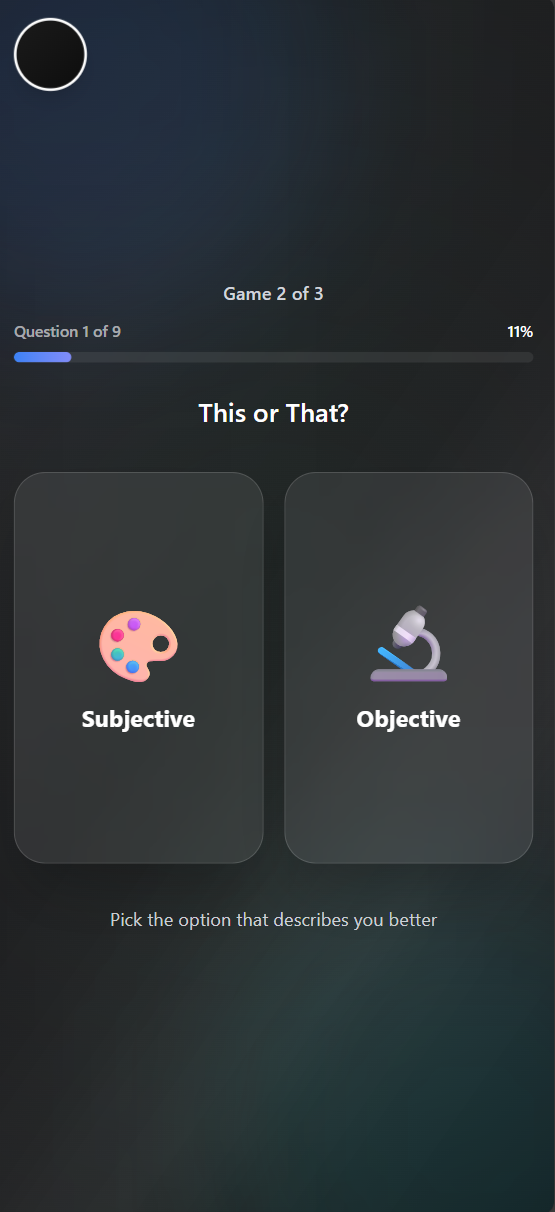
\includegraphics[width=0.75\textwidth,height=0.75\textheight,keepaspectratio]{Figures/game_2_this_or_that.png}
    \caption{Game 2: This or That interface.}
    \label{fig:game2}
\end{figure}

% TODO: Explain how Game 2 responses are used mechanically in Stage 1 and Stage 2 matching.
% Currently the text says Game 2 feeds both stages but never explains the mapping.
% A sentence or two on how these dimension scores get weighted against cluster profiles
% would close this gap without exposing the full algorithm.

\textbf{Game 3: Select 3} presents the student with eight keywords drawn from each of their matched clusters. The student selects their top 3. The keyword sets are cluster-specific (see Appendix~\ref{app:games} for the full list).

\begin{figure}[h]
    \centering
    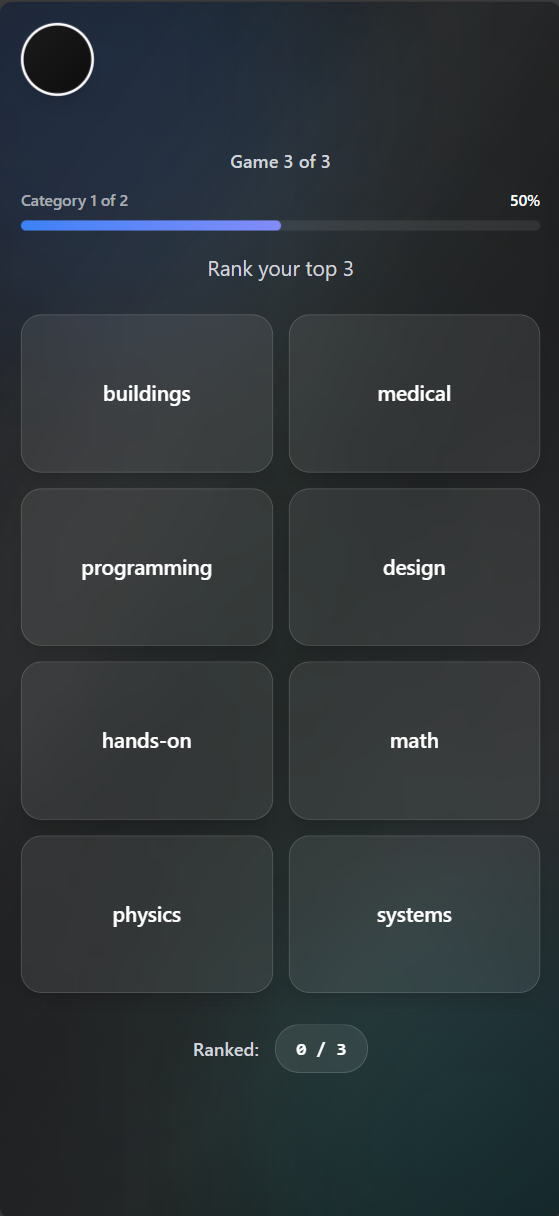
\includegraphics[width=0.75\textwidth,height=0.75\textheight,keepaspectratio]{Figures/game_3_select_3.png}
    \caption{Game 3: Select 3 interface.}
    \label{fig:game3}
\end{figure}

\section{Deployment and Iteration}

% TODO: Add at least one concrete example of what changed between versions and why.
% "Six iterations" without any detail reads as a number without a story. Even one
% example (e.g., a game mechanic that was added, removed, or reworded based on feedback)
% would make the iteration claim substantive.

The current version of MajorMatch represents the sixth iteration developed over several months. Feedback driving each revision came from qualitative user interviews, user retention rates, and quantitative signals including star ratings and thumbs up/down responses. The latest version has been used more than 950 times.

The core MajorMatch framework has also been extended to custom versions, including a careers-focused variant and university-specific versions that link recommendations back to actual catalog offerings.

% TODO: Add an implications/discussion paragraph closing the chapter. The chapter
% currently ends on extensions without connecting back to the thesis argument.
% One paragraph on what deployment validates -- that cluster-based interest elicitation
% is viable in practice and that the semantic groupings hold up under real user interaction
% -- would tie Chapter 4 back to Chapter 3 and set up the conclusion.

\newpage
